\documentclass[border=5pt]{standalone}

\usepackage{amsmath,amssymb}
\def\pgfsysdriver{pgfsys-dvisvgm.def}
\usepackage{tikz}
\usetikzlibrary{arrows.meta,calc,positioning}

\definecolor{queryblue}{RGB}{210,224,242}
\definecolor{weightblue}{RGB}{232,239,247}
\definecolor{headgreen}{RGB}{221,236,224}
\definecolor{concatviolet}{RGB}{232,224,243}
\definecolor{outputgold}{RGB}{247,236,201}

\tikzset{
  >=Latex,
  flow/.style={->,draw=black,line width=0.7pt},
  flowline/.style={draw=black,line width=0.7pt},
  operator/.style={
    draw=black,
    rectangle,
    minimum height=8.5mm,
    minimum width=18mm,
    inner sep=2pt,
    align=center,
    font=\footnotesize
  },
  headbox/.style={
    draw=black,
    rectangle,
    minimum height=12mm,
    minimum width=30mm,
    inner sep=3pt,
    align=center,
    font=\footnotesize
  },
  dim/.style={font=\scriptsize},
  note/.style={font=\scriptsize,align=center},
  panel/.style={font=\bfseries\large,anchor=west}
}

\newcommand{\gridmatrix}[8]{%
  \begin{scope}[shift={(#1,#2)}]
    \filldraw[fill=#7,draw=black,line width=0.55pt] (0,0) rectangle (#3,#4);
    \pgfmathsetmacro{\colstep}{#3/#6}
    \pgfmathsetmacro{\rowstep}{#4/#5}
    \foreach \col in {1,...,\numexpr#6-1\relax} {
      \draw[line width=0.4pt] (\col*\colstep,0) -- (\col*\colstep,#4);
    }
    \foreach \row in {1,...,\numexpr#5-1\relax} {
      \draw[line width=0.4pt] (0,\row*\rowstep) -- (#3,\row*\rowstep);
    }
    \node[font=\bfseries,above=1.6mm] at (#3/2,#4) {#8};
  \end{scope}
}

\begin{document}
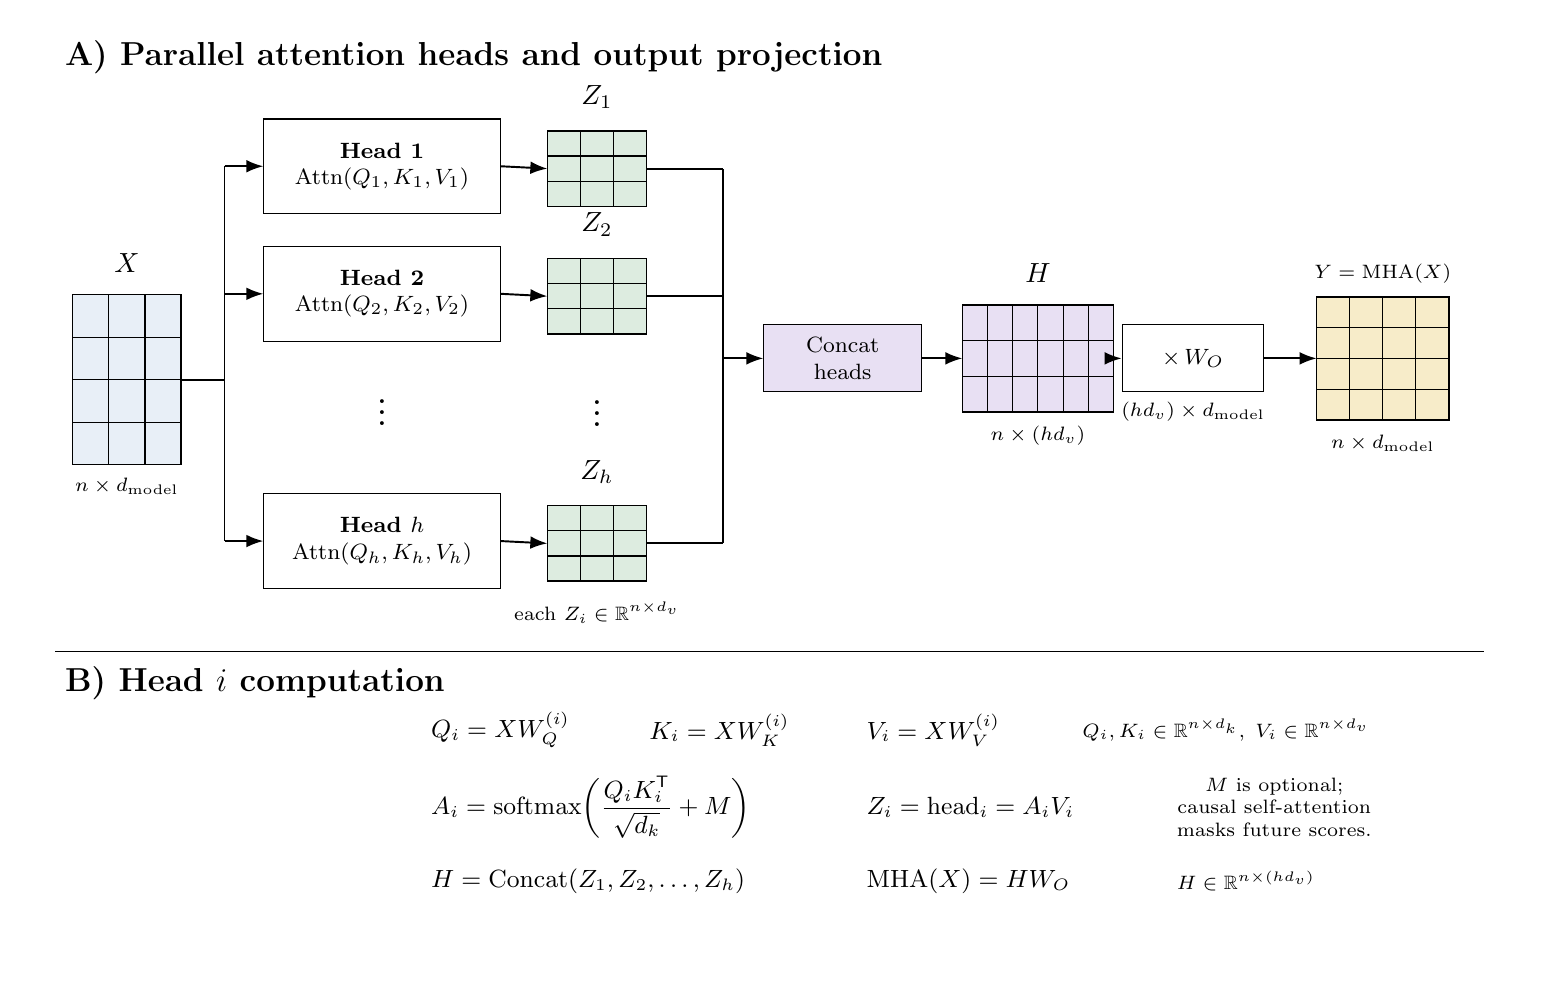
\begin{tikzpicture}[x=1cm,y=1cm]
  \fill[white] (-0.35,-2.75) rectangle (18.85,9.10);

  % Panel A
  \node[panel] at (0,8.72) {A) Parallel attention heads and output projection};

  % Shared input
  \gridmatrix{0.22}{3.55}{1.38}{2.16}{4}{3}{weightblue}{$X$}
  \node[dim] at (0.91,3.28) {$n \times d_{\mathrm{model}}$};
  \coordinate (xfan) at (2.15,4.63);
  \draw[flowline] (1.60,4.63) -- (xfan);
  \draw[flowline] (xfan) -- (2.15,7.34);
  \draw[flowline] (xfan) -- (2.15,2.58);

  % Parallel heads
  \node[headbox] (headone) at (4.15,7.34)
    {\textbf{Head 1}\\$\operatorname{Attn}(Q_1,K_1,V_1)$};
  \node[headbox] (headtwo) at (4.15,5.72)
    {\textbf{Head 2}\\$\operatorname{Attn}(Q_2,K_2,V_2)$};
  \node[font=\Large] at (4.15,4.32) {$\vdots$};
  \node[headbox] (headh) at (4.15,2.58)
    {\textbf{Head $h$}\\$\operatorname{Attn}(Q_h,K_h,V_h)$};

  \draw[flow] (2.15,7.34) -- (headone.west);
  \draw[flow] (2.15,5.72) -- (headtwo.west);
  \draw[flow] (2.15,2.58) -- (headh.west);

  % Head outputs
  \gridmatrix{6.25}{6.83}{1.26}{0.96}{3}{3}{headgreen}{$Z_1$}
  \gridmatrix{6.25}{5.21}{1.26}{0.96}{3}{3}{headgreen}{$Z_2$}
  \node[font=\Large] at (6.88,4.30) {$\vdots$};
  \gridmatrix{6.25}{2.07}{1.26}{0.96}{3}{3}{headgreen}{$Z_h$}
  \node[dim] at (6.88,1.67) {each $Z_i\in\mathbb{R}^{n\times d_v}$};

  \draw[flow] (headone.east) -- (6.25,7.31);
  \draw[flow] (headtwo.east) -- (6.25,5.69);
  \draw[flow] (headh.east) -- (6.25,2.55);

  % Concatenate head outputs
  \coordinate (headbus) at (8.48,4.90);
  \draw[flowline] (7.51,7.31) -- (8.48,7.31);
  \draw[flowline] (7.51,5.69) -- (8.48,5.69);
  \draw[flowline] (7.51,2.55) -- (8.48,2.55);
  \draw[flowline] (8.48,2.55) -- (8.48,7.31);

  \node[operator,minimum width=20mm,fill=concatviolet] (concat) at (10.00,4.90)
    {$\operatorname{Concat}$\\heads};
  \draw[flow] (headbus) -- (concat.west);

  \gridmatrix{11.52}{4.22}{1.92}{1.36}{3}{6}{concatviolet}{$H$}
  \node[dim] at (12.48,3.92) {$n \times (h d_v)$};
  \draw[flow] (concat.east) -- (11.52,4.90);

  % Output projection
  \node[operator,minimum width=18mm] (wo) at (14.45,4.90) {$\times\,W_O$};
  \draw[flow] (13.44,4.90) -- (wo.west);
  \node[dim] at (14.45,4.22) {$(h d_v) \times d_{\mathrm{model}}$};

  \gridmatrix{16.02}{4.12}{1.68}{1.56}{4}{4}{outputgold}{}
  \node[dim] at (16.86,3.82) {$n \times d_{\mathrm{model}}$};
  \node[dim] at (16.86,5.98) {$Y=\operatorname{MHA}(X)$};
  \draw[flow] (wo.east) -- (16.02,4.90);

  % Panel divider
  \draw[line width=0.55pt] (0,1.18) -- (18.15,1.18);

  % Panel B
  \node[panel] at (0,0.78) {B) Head $i$ computation};

  \node[font=\small,anchor=west] at (4.65,0.18)
    {$Q_i=XW_Q^{(i)}$};
  \node[font=\small,anchor=west] at (7.42,0.18)
    {$K_i=XW_K^{(i)}$};
  \node[font=\small,anchor=west] at (10.18,0.18)
    {$V_i=XW_V^{(i)}$};
  \node[dim,anchor=west] at (12.92,0.18)
    {$Q_i,K_i\in\mathbb{R}^{n\times d_k},\;V_i\in\mathbb{R}^{n\times d_v}$};

  \node[font=\small,anchor=west] at (4.65,-0.80)
    {$\displaystyle A_i=\operatorname{softmax}\!\left(\frac{Q_iK_i^{\mathsf T}}{\sqrt{d_k}}+M\right)$};
  \node[font=\small,anchor=west] at (10.18,-0.80)
    {$Z_i=\operatorname{head}_i=A_iV_i$};
  \node[note,anchor=west] at (14.12,-0.80)
    {$M$ is optional;\\causal self-attention\\masks future scores.};

  \node[font=\small,anchor=west] at (4.65,-1.74)
    {$H=\operatorname{Concat}(Z_1,Z_2,\ldots,Z_h)$};
  \node[font=\small,anchor=west] at (10.18,-1.74)
    {$\operatorname{MHA}(X)=HW_O$};
  \node[dim,anchor=west] at (14.12,-1.74)
    {$H\in\mathbb{R}^{n\times(hd_v)}$};
\end{tikzpicture}
\end{document}
